\documentclass[10pt, aspectratio=169]{beamer}
\usetheme{Madrid}
\usecolortheme{seahorse}

\usepackage{graphicx}
\usepackage{booktabs}
\usepackage{amsmath}
\usepackage{hyperref}
\usepackage{caption}
\usepackage{tabularx}
\usepackage{multicol}

% Adjust caption font size
\captionsetup{font=scriptsize}

\title[RL for Music Emotion Therapy]{Reinforcement Learning using EEG Signals for \\Therapeutic Use of Music in Emotion Management}
\author[Nagwani, Gautam, Manhar]{\textbf{Sahil Nagwani (U23AI106)} \and \textbf{Vishal Gautam (U23AI127)} \and \textbf{Prakriti Manhar (U23AI114)}}
\institute{Department of Artificial Intelligence}
\date{\today}

\begin{document}

% -----------------------------------------------------------
% Slide 1: Title Page
% -----------------------------------------------------------
\begin{frame}
    \titlepage
\end{frame}

% -----------------------------------------------------------
% Slide 2: Outline
% -----------------------------------------------------------
\begin{frame}{Presentation Outline}
    \tableofcontents
\end{frame}

% -----------------------------------------------------------
% Slide 3: The Hook & Motivation
% -----------------------------------------------------------
\section{Motivation}
\begin{frame}{The Hook: Why This Research Matters}
    \textbf{Music as Therapy: A Gateway to Emotion Regulation}
    \begin{itemize}
        \item \textbf{Global Mental Health Challenge}: Mood disorders and emotional dysregulation are prevalent global issues. Traditional therapies often require intensive clinical supervision.
        \item \textbf{The Power of Music}: Music has a profound, scientifically proven capability to modulate human emotions, acting directly on the limbic system to alter affective states.
        \item \textbf{Why EEG?}: Electroencephalography (EEG) provides an objective, real-time window into cognitive and emotional brain dynamics, bypassing flawed subjective self-reports.
        \item \textbf{The Need for Personalization}: Human responses to music are highly subjective. A one-size-fits-all approach is ineffective.
        \item \textbf{The RL Shift}: We introduce Reinforcement Learning (RL) to transition from static music recommendations to an \textit{adaptive, personalized therapeutic intervention} that actively guides a user's emotional state natively.
    \end{itemize}
\end{frame}

% -----------------------------------------------------------
% Slide 4: Problem Statement
% -----------------------------------------------------------
\section{Problem Statement}
\begin{frame}{Problem Statement \& Research Question}
    \textbf{The Problem:} \\
    Current affective brain-computer interfaces (aBCI) are largely reactive—they identify how a user feels. There is a critical gap in building \textit{active, closed-loop systems} capable of autonomously driving a person from a wide range of initial states (e.g., negative, sad, anger) to a desired positive target (e.g., happiness) using dynamic stimuli selection.

    \vspace{0.5cm}
    \textbf{Research Questions:}
    \begin{enumerate}
        \item Can a Reinforcement Learning agent effectively learn to select a sequence of music clips that navigates a user's emotional state toward a specific target ('happy') within a 2D Valence-Arousal space?
        \item How do different RL paradigms (Q-Learning, SARSA, Double Q-Learning, Double SARSA) compare across \textbf{all 8 basal starting emotions}?
        \item What is the impact of explicit reward shaping on mitigating emotional stagnation loops?
    \end{enumerate}
\end{frame}

% -----------------------------------------------------------
% Slide 5: Previous Work
% -----------------------------------------------------------
\section{Previous Work}
\begin{frame}{Previous Work \& Context}
    \begin{itemize}
        \item \textbf{Emotion Recognition (DEAP Dataset)}: Prior studies heavily rely on the DEAP dataset for emotion recognition using physiological signals. Most focus purely on classification (e.g., SVMs, simple LSTMs).
        \item \textbf{Dutta et al. (2020)}: Proposed an initial Q-Learning framework for music emotion regulation using a discretized $20 \times 20$ Valence-Arousal space. We use this as our foundational benchmark.
        \item \textbf{Limitations of Current RL in Therapy}:
        \begin{itemize}
            \item \textbf{Overestimation Bias}: High variance in human subjects makes standard Q-learning prone to overestimating the therapeutic value of certain clips.
            \item \textbf{Exploration Stagnation}: Agents often repeatedly choose clips that effect no emotional change (loops).
        \end{itemize}
        \item \textbf{Our Contribution}: We expand upon previous work by implementing a rigorous comparative analysis of four algorithms, evaluating convergence strictly using a rigorous $\leq 20^\circ$ angular error threshold, and modeling performance natively across \textit{every} starting emotion category.
    \end{itemize}
\end{frame}

% -----------------------------------------------------------
% Slide 6: Methods & Data Sources
% -----------------------------------------------------------
\section{Methods \& Setup}
\begin{frame}{Methods: Data \& Environment Modeling}
    \begin{columns}
        \column{0.55\textwidth}
        \textbf{Dataset: DEAP}
        \begin{itemize}
            \item 32 participants, 40 music video trials per subject (1 minute each).
            \item Features: EEG signals processed to map directly to Valence and Arousal dimensions.
        \end{itemize}
        \textbf{State Space ($\mathcal{S}$)}
        \begin{itemize}
            \item Continuous 2D Valence-Arousal space, discretized into a $20 \times 20$ grid (400 states).
            \item 15 fine-grained emotions mapped into 8 main clusters.
        \end{itemize}
        \textbf{Action Space ($\mathcal{A}$) \& Transitions}
        \begin{itemize}
            \item 1240 possible music clips to choose from.
            \item Transitions are modeled additively based strictly on empirical DEAP EEG vectors.
        \end{itemize}
        \column{0.45\textwidth}
        \centering
        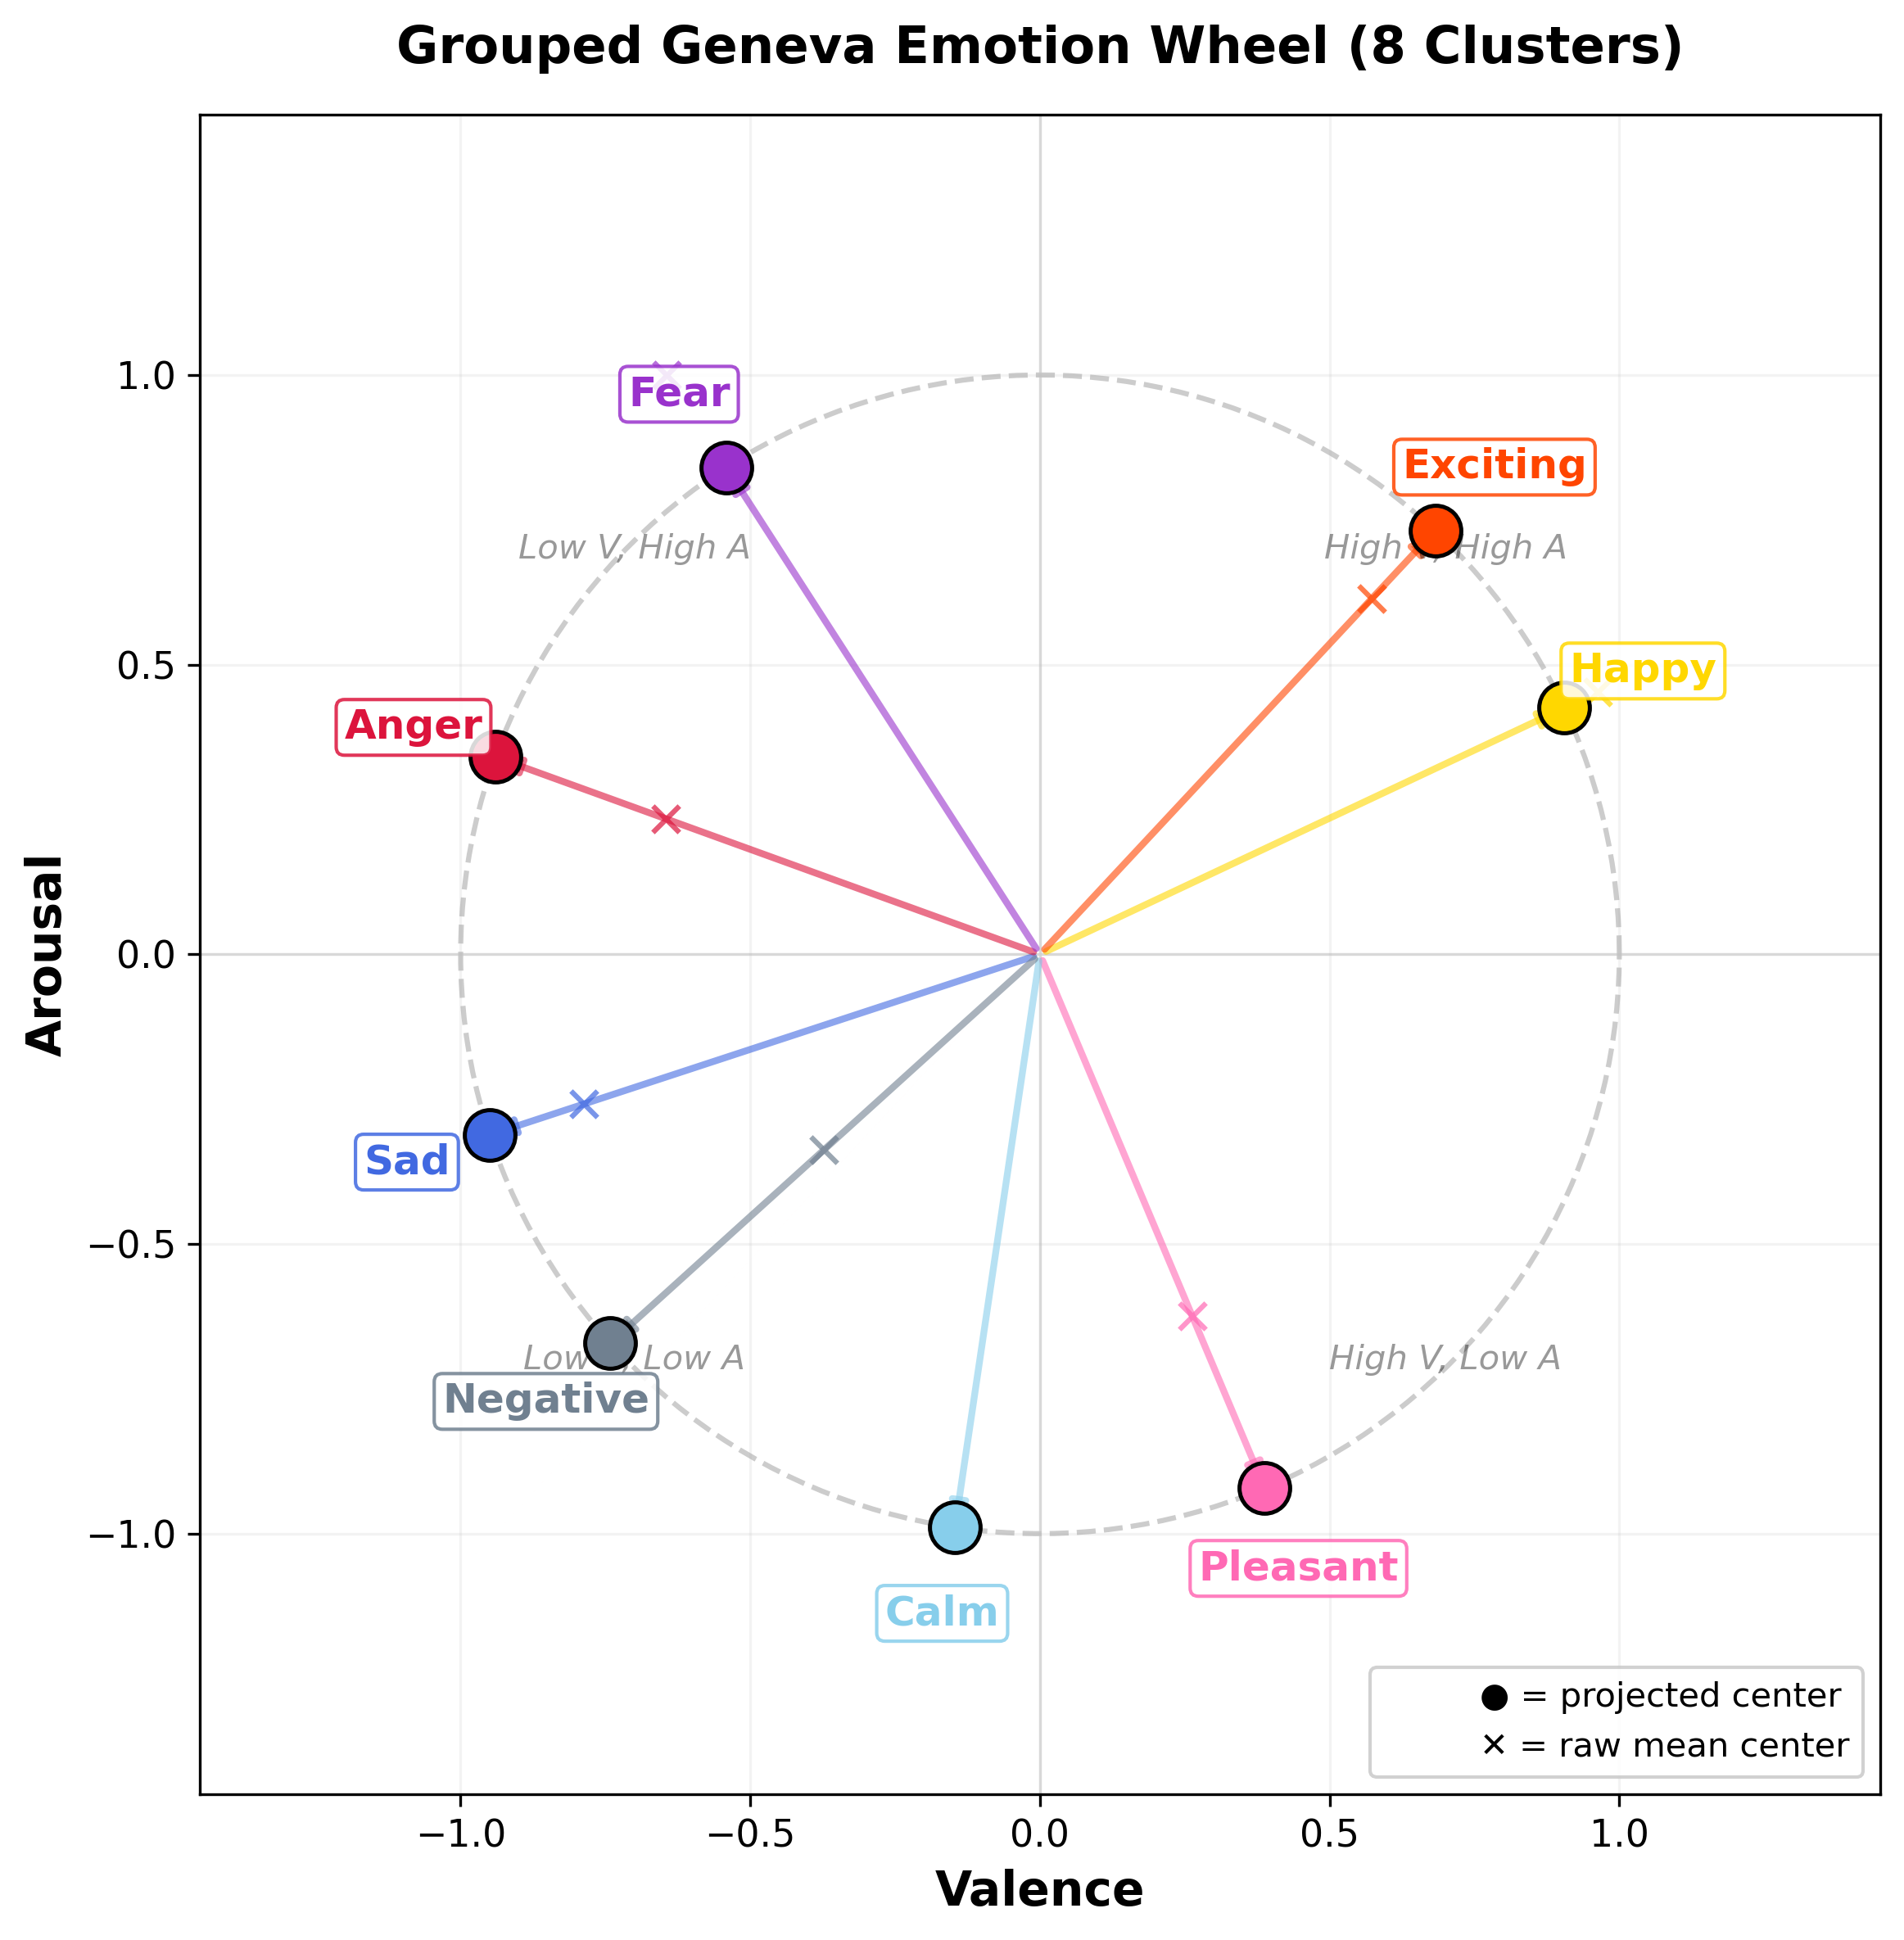
\includegraphics[width=\linewidth, height=4.5cm, keepaspectratio]{results_compare/grouped_gew.png}
        \captionof{figure}{Our 8-Cluster Geneva Emotion Wheel}
    \end{columns}
\end{frame}

% -----------------------------------------------------------
% Slide 7: Reward Design
% -----------------------------------------------------------
\begin{frame}{Experimental Setup: Strict Convergence \& Awards}
    \textbf{Target Emotion}: 'Happy' (High Valence, Moderate Arousal). \\
    \textbf{Strict Convergence Criterion}: Angular Error $\leq 20^\circ$ ONLY. (We discarded "closest cluster" matching to ensure absolute rigorous clinical viability).
    
    \vspace{0.4cm}
    \textbf{Reward Function Formulation:}
    \begin{equation*}
        R_{base} = 1.0 \text{ if angle towards target is favorable, else } 0.0
    \end{equation*}
    \begin{equation*}
        R_{terminal} = +10.0 \text{ (Bonus if Goal reached)}
    \end{equation*}
    
    \vspace{0.2cm}
    \textbf{Stagnation Penalty ($\lambda$)}:
    \begin{equation*}
        \Phi(s, s') = 
        \begin{cases} 
        -100 & \text{if } s = s' \text{ (No emotional change)} \\
        0 & \text{otherwise}
        \end{cases}
    \end{equation*}
    This enforces a hard penalty for zero-transition actions, ensuring the agent continually explores rather than trapping the subject in a stable but depressing emotional baseline.
\end{frame}

% -----------------------------------------------------------
% Slide 8: The Algorithms Overview
% -----------------------------------------------------------
\section{Algorithms}
\begin{frame}{The Tested Reinforcement Learning Algorithms}
    \begin{itemize}
        \item \textbf{Q-Learning (Off-Policy)}: Evaluates the optimal absolute path. \\
        Update: $Q(s, a) \leftarrow Q(s, a) + \alpha [ r + \gamma \max_{a'} Q(s', a') + \Phi(s, s') - Q(s, a) ]$
        
        \item \textbf{SARSA (On-Policy)}: Evaluates the actual exploratory path taken. \\
        Update: $Q(s, a) \leftarrow Q(s, a) + \alpha [ r + \gamma Q(s', a') + \Phi(s, s') - Q(s, a) ]$
        
        \item \textbf{Double Q-Learning (Off-Policy)}: Decouples action selection from value estimation to prevent maximization bias (using tables $Q^A, Q^B$). \\
        Target: $r + \gamma Q^B(s', \arg\max_{a} Q^A(s', a)) + \Phi(s, s')$
        
        \item \textbf{Double SARSA (On-Policy)}: The on-policy equivalent of dual-table isolation. Evaluates actual actions but queries the secondary decoupled table.
    \end{itemize}
\end{frame}

% -----------------------------------------------------------
% Slide 9: Master Results Overview
% -----------------------------------------------------------
\section{Visual Results}
\begin{frame}{Overall Performance Across All States (Convergence: $\leq 20^\circ$)}
    Due to our aggressive strict limitation ($\leq 20^\circ$), convergence is clinically precise.
    
    \begin{table}[]
        \centering
        \caption{Success Rate out of 32 Subjects (With Reward Shaping $\lambda=-100$)}
        \resizebox{0.9\columnwidth}{!}{%
        \begin{tabular}{l c c|c c}
            \toprule
            \textbf{Start Emotion} & \textbf{Q-Learning} & \textbf{Double Q-Learning} & \textbf{SARSA} & \textbf{Double SARSA} \\
            \midrule
            Happy & 11/32 & \textbf{13/32} & 8/32 & 12/32 \\
            Pleasant & 11/32 & \textbf{15/32} & 4/32 & 3/32 \\
            Exciting & \textbf{15/32} & 14/32 & 9/32 & 11/32 \\
            \midrule
            Calm & \textbf{11/32} & 12/32 & 4/32 & 3/32 \\
            Sad & 5/32 & \textbf{6/32} & 2/32 & 4/32 \\
            Negative & 5/32 & \textbf{11/32} & 3/32 & 4/32 \\
            \midrule
            Anger & 11/32 & \textbf{17/32} & 8/32 & 8/32 \\
            Fear & \textbf{24/32} & 22/32 & 8/32 & 5/32 \\
            \bottomrule
        \end{tabular}
        }
    \end{table}
    \textbf{Overall Trend:} Double Q-Learning consistently proves to be the most robust architecture across nearly all diverse starting states, particularly when starting in deep negative quadrants.
\end{frame}

% -----------------------------------------------------------
% Slide 10: Emotion Highlight - Anger
% -----------------------------------------------------------
\begin{frame}{State Analysis: Starting from ANGER}
    \textbf{Anger:} A high-arousal, highly negative state. Moderately difficult to navigate directly to Happy (high-arousal, positive).
    
    \begin{columns}
        \column{0.5\textwidth}
        \centering
        
\includegraphics[width=\linewidth, height=3.5cm, keepaspectratio]{results/anger/compare_convergence_bar_with.png} \\
        \footnotesize{Convergence Bars (Start: Anger, With Shaping)}
        \column{0.5\textwidth}
        \centering
        
\includegraphics[width=\linewidth, height=3.5cm, keepaspectratio]{results/anger/compare_angular_error_with.png} \\
        \footnotesize{Mean Angular Error decay per clip}
    \end{columns}
    
    \vspace{0.3cm}
    \textbf{Key Findings (Anger):}
    \begin{itemize}
        \item Double Q-Learning achieves the highest success (17/32 strict convergences).
        \item It suppresses the chaotic overestimation bias seen in standard Q-Learning, yielding an explicitly smoother angular descent curve by Clip 6.
    \end{itemize}
\end{frame}

% -----------------------------------------------------------
% Slide 11: Emotion Highlight - Fear & Negative
% -----------------------------------------------------------
\begin{frame}{State Analysis: FEAR vs NEGATIVE}
    \begin{columns}
        \column{0.5\textwidth}
        \textbf{Starting from FEAR}
        \begin{itemize}
            \item Q-Learning dominates (24/32).
            \item Fear is neighboring Exciting. The agent quickly masters the High-Arousal traversal into the Happy zone.
            \item \textit{Observation}: On-policy algorithms (SARSA) collapsed almost completely (8/32), failing to explore the correct bridge.
        \end{itemize}
        \centering
        
\includegraphics[width=\linewidth, height=2.5cm, keepaspectratio]{results/fear/compare_convergence_bar_with.png}
        
        \column{0.5\textwidth}
        \textbf{Starting from NEGATIVE}
        \begin{itemize}
            \item The hardest traversal state globally.
            \item Double Q-Learning (11/32) is uniquely successful. Standard QL falters (5/32).
            \item \textit{Observation}: Extracting a user from deep low-arousal, high-negative states is incredibly noisy. Double QL's conservative step estimation shines here.
        \end{itemize}
        \centering
        
\includegraphics[width=\linewidth, height=2.5cm, keepaspectratio]{results/negative/compare_convergence_bar_with.png}
    \end{columns}
\end{frame}

% -----------------------------------------------------------
% Slide 12: Emotion Highlight - Sadness & Calm
% -----------------------------------------------------------
\begin{frame}{State Analysis: The Low Arousal Regimes (Sad \& Calm)}
    \begin{columns}
        \column{0.5\textwidth}
        \centering
        
\includegraphics[width=\linewidth, height=4cm, keepaspectratio]{results/sad/compare_angular_error_with.png} \\
        \footnotesize{Angular Error Decay (Start: SAD)}
        \column{0.5\textwidth}
        \textbf{Challenges in Low Arousal:}
        \begin{itemize}
            \item \textbf{Sadness}: Very poor overall performance structurally. Raising a user's arousal levels (to reach 'Happy') using only music clips triggers immense variance. Highest mean errors across all groups.
            \item \textbf{Calm}: A positive but low-arousal state. Often treated as a "false positive trap" by on-policy exploratory agents, getting stuck near Pleasant instead of pushing to Happy.
        \end{itemize}
    \end{columns}
\end{frame}

% -----------------------------------------------------------
% Slide 13: Reward Shaping Effect
% -----------------------------------------------------------
\begin{frame}{The Transformative Impact of Reward Shaping Constraints}
    We implemented a stagnation penalty ($\lambda = -100$) where $\Phi(s,s') \neq 0$ if the emotional state did not transition.
    
    \begin{columns}
        \column{0.5\textwidth}
        \centering
        
\includegraphics[width=\linewidth, height=4cm, keepaspectratio]{results/anger/compare_shaping_convergence.png} \\
        \footnotesize{Shaping Impact on Anger Convergence}
        \column{0.5\textwidth}
        \textbf{Why it works:}
        \begin{itemize}
            \item \textbf{Standard RL} gets repeatedly rewarded or neutrally ignored for remaining in identical states.
            \item \textbf{Explicit Penalties} force the agent into deep exploration across the Valence/Arousal axis. 
            \item Visually, the green bars (With shaping) universally eclipse red bars (Without shaping) out of the 32 subjects across all algorithms.
        \end{itemize}
    \end{columns}
\end{frame}

% -----------------------------------------------------------
% Slide 14: Implications & Limitations
% -----------------------------------------------------------
\section{Discussion}
\begin{frame}{Interpretation of Findings \& Limitations}
    \textbf{Answering the Research Questions}
    \begin{itemize}
        \item \textbf{Yes, RL Works}: The closed-loop formulation successfully modulated theoretical user states from deep negative bases to a $\leq 20^\circ$ precision target using only EEG-derived mappings.
        \item \textbf{Off-Policy is Superior}: The extreme unpredictability of human emotion makes \textit{exploratory consequence} highly dangerous. Q-Learning and DQQ-Learning (which evaluate absolute optimal values) consistently outperformed SARSA (which evaluates exploratory paths).
    \end{itemize}
    
    \vspace{0.4cm}
    \textbf{Limitations}
    \begin{itemize}
        \item \textbf{Strict Convergence Penalty}: By using $\leq 20^\circ$ instead of "closest centroid matching", our raw quantitative hit rates dropped, highlighting the difficulty in achieving \textit{perfect} localized valence/arousal targets.
        \item \textbf{Data Mapping Constraint}: The transition tables are reliant on existing discrete human feedback trials from DEAP, which may not generalize seamlessly to prolonged continuous temporal stimulation.
    \end{itemize}
\end{frame}

% -----------------------------------------------------------
% Slide 15: Future Work
% -----------------------------------------------------------
\begin{frame}{Next Steps \& Future Integrations}
    \textbf{Integrating a Deep Sequential Emotion Classifier (Bidirectional LSTM)}
    
    While the RL agent mapped the policy trajectory impressively well, maintaining real-time accuracy on exactly where the active brain state sits natively is challenging with pure EEG frequency bands.
    
    \begin{itemize}
        \item \textbf{Goal}: Train a bidirectional LSTM across temporal EEG windows to serve as an intermediary "state observer" for the RL agent. 
        \item \textbf{Effect}: Vastly improves noise resiliency within the state vector before it is handed to the Q-tables for action selection.
        \item \textbf{Real-World Loop}: Establish a BCI lab trial mapping real-time OpenBCI equipment to the trained Double Q-Learning model for human-in-the-loop therapy verification.
    \end{itemize}
\end{frame}

% -----------------------------------------------------------
% Slide 16: End
% -----------------------------------------------------------
\begin{frame}
    \centering
    \Huge \textbf{Thank You!} \\
    \vspace{1cm}
    \large Questions?
\end{frame}

\end{document}
